\section{Triboson Background}
\label{SectionTriboson}

\vspace{7mm}

\begin{figure}[htb]
    \centering
    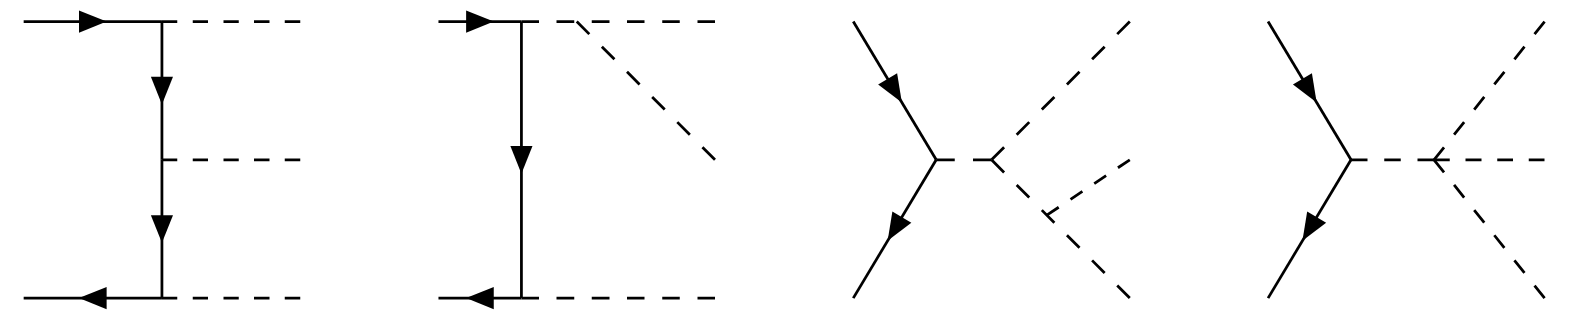
\includegraphics[scale=0.2]{TribosonGeneric.png}
    \caption{}
    % https://www.ugr.es/~pittau/talk_granada_2008.pdf
    \label{fig:TriGeneric}
\end{figure}


A representative example of each process is shown in next sections. 

The qq-> VVV production is dominant with respect the gluon production


\subsection{An example of WWW production}

\vspace{7mm}

\begin{figure}[htb]
    \centering
    \begin{fmffile}{WWW}
    \begin{fmfgraph*}(100,60)
      % # ins/outs
      \fmfleft{i1,i2}
      \fmfright{o1,o2,o3}
      \fmftop{t}
      \fmfbottom{b}
      % ins
      \fmf{fermion}{i2,v1}
      \fmf{fermion}{v1,i1}
      % mediators
      \fmf{photon, label=$W^{\pm}$}{v1,v2}
      \fmf{photon}{v2,o2}
      \fmflabel{$W^{\mp}$}{o2}
      \fmffreeze
      \fmf{phantom}{v2,o1}
      %\fmf{phantom}{v2,o2}
      \fmf{phantom}{v2,o3}
      \fmffreeze
      \fmf{photon,tension=0}{v2,o1}
      \fmf{photon,tension=0}{v2,o3}
      % labels
      \fmflabel{$q$}{i2}
      \fmflabel{$\overline{q}'$}{i1}
      \fmflabel{$W^{\pm}$}{o3}
      \fmflabel{$W^{\pm}$}{o1}
    \end{fmfgraph*}
    \end{fmffile}
    \vspace{3mm}
    \caption{}
    \label{fig:WWW}
    % https://open.bu.edu/handle/2144/17737
\end{figure}



\subsection{An example of WWZ production}


\vspace{7mm}


\begin{figure}[htb]
    \centering
    \begin{fmffile}{WWZ}
    \begin{fmfgraph*}(100,60)
    \fmfstraight
    \fmfleft{i2,i1}
    \fmfright{o1,l1,l2}
    % skeleton
    \fmf{phantom}{i1,v1}
    \fmf{phantom}{v1,l1}
    \fmf{phantom, tension=0.3}{v1,v2}
    \fmf{phantom}{i2,v2}
    \fmf{phantom}{v2,o1}
    \fmffreeze
    % W + jets
    \fmfshift{5 right}{l1,l2}
    \fmfshift{20 left}{o1}
    % quarks
    \fmflabel{$q$}{i1}
    \fmflabel{$\overline{q}$}{i2}
    \fmf{fermion}{i1,v1,v2,i2}
    % W boson
    \fmf{boson,tension=1.2,label=$Z^0/\gamma$,label.side=left}{v1,z}
    \fmf{photon}{v2,o1}
    \fmflabel{$Z^0$}{o1}
    % leptons
    \fmflabel{$W^+$}{l1}
    \fmflabel{$W^-$}{l2}
    \fmf{photon}{l1,z,l2}
    \end{fmfgraph*}
    \end{fmffile}
    \vspace{3mm}
    \caption{}
    \label{fig:WWZ}
\end{figure}

% https://arxiv.org/pdf/1310.6159.pdf

\subsection{An example of WZZ production}
\vspace{7mm}

\begin{figure}[htb]
    \centering
    \begin{fmffile}{WZZ}
    \begin{fmfgraph*}(100,60)
    %\fmfstraight
    \fmfleft{i1,i3} 
    \fmfright{o1,o2,o3}
    \fmf{fermion}{v1,i1}
    \fmf{fermion}{i3,v3}
    \fmf{photon}{v3,o3}
    \fmf{photon}{v1,o1}
    \fmffreeze
    \fmf{fermion, label.side=left}{v3,v2,v1}
    \fmffreeze
    \fmf{photon, tension= 1.1}{v2,o2}
    \fmflabel{$\overline{q}$}{i1}
    \fmflabel{$q$'}{i3}
    \fmflabel{$W^{\pm}$}{o2}
    \fmflabel{$Z^0$}{o1}
    \fmflabel{$Z^0$}{o3}
    \end{fmfgraph*}
    \end{fmffile}
    \vspace{3mm}
    \caption{}
    \label{fig:WZZ}
\end{figure}

\subsection{An example of ZZZ production}

\vspace{7mm}

\begin{figure}[htb]
    \centering
    \begin{fmffile}{ZZZ}
  \begin{fmfgraph*}(100,60)
    \fmfstraight
    \fmfleft{i2,m,i1}
    \fmfright{o2,l2,l1}
    % skeleton
    \fmf{phantom,tension=1.0}{i1,v1}
    \fmf{phantom,tension=1.0}{v2,l1}
    \fmf{phantom,tension=1.5}{v1,v2}
    \fmf{phantom,tension=1.0}{i2,v1}
    \fmf{phantom,tension=1.0}{v2,o2}
    \fmf{phantom,tension=0.6}{i1,t1,m}
    \fmf{phantom,tension=0.6}{t1,LQ}
    \fmf{phantom,tension=2.0}{l1,LQ,l2}
    \fmffreeze
    % gluon + quarks
    \fmf{phantom,tension=5.0}{i1,g} % shorten leg
    \fmf{phantom,tension=5.0}{i2,q} % shorten leg
    \fmf{phantom,tension=5.0}{o2,l} % shorten leg
    \fmf{fermion}{g,v1}
    \fmf{fermion}{v1,q}
    \fmf{photon,label=$Z^0$,label.side=right}{v1,v2}
    \fmf{photon}{v2,l}
    \fmflabel{$q$}{g}
    \fmflabel{$\overline{q}$}{q}
    \fmflabel{$Z^0$}{l}
    % LQ
    \fmf{dashes,tension=1.2,label=H,label.side=left}{v2,LQ}
    % LQ -> lepton + quark
    \fmf{photon}{l2,LQ,l1}
    \fmfshift{20 right}{l1,l2}
    \fmflabel{$Z^0$}{l1}
    \fmflabel{$Z^0$}{l2}
  \end{fmfgraph*}
\end{fmffile}
\vspace{3mm}
    \caption{}
    \label{fig:ZZZ}
\end{figure}